% bei Standalone in documentclass noch:
% \RequirePackage{luatex85}

\documentclass[captions=tableheading, titlepage= firstiscover, parskip = half , bibliography=totoc]{scrartcl}
%paper = a5 für andere optinen
% titlepage= firstiscover
% bibliography=totoc für bibdateien
% parskip=half  Veränderung um Absätze zu verbessern

\usepackage{scrhack} % nach \documentclass
\usepackage[aux]{rerunfilecheck}
\usepackage{polyglossia}
\usepackage[style=numeric, backend=biber]{biblatex} % mit [style = alphabetic oder numeric] nach polyglossia
\addbibresource{lit.bib}
\setmainlanguage{german}

\usepackage[autostyle]{csquotes}
\usepackage{amsmath} % unverzichtbare Mathe-Befehle
\usepackage{amssymb} % viele Mathe-Symbole
\usepackage{mathtools} % Erweiterungen für amsmath
\usepackage{fontspec} % nach amssymb
% muss ins document: \usefonttheme{professionalfonts} % für Beamer Präsentationen
\usepackage{longtable}

\usepackage[
math-style=ISO,    % \
bold-style=ISO,    % |
sans-style=italic, % | ISO-Standard folgen
nabla=upright,     % |
partial=upright,   % /
]{unicode-math} % "Does exactly what it says on the tin."
\setmathfont{Latin Modern Math}
% \setmathfont{Tex Gyre Pagella Math} % alternativ

\usepackage[
% die folgenden 3 nur einschalten bei documenten
locale=DE,
separate-uncertainty=true, % Immer Fehler mit ±
per-mode=symbol-or-fraction, % m/s im Text, sonst \frac
]{siunitx}

% alternativ:
% per-mode=reciprocal, % m s^{-1}
% output-decimal-marker=., % . statt , für Dezimalzahlen

\usepackage[
version=4,
math-greek=default,
text-greek=default,
]{mhchem}

\usepackage[section, below]{placeins}
\usepackage{caption} % Captions schöner machen
\usepackage{graphicx}
\usepackage{grffile}
\usepackage{subcaption}

% \usepackage{showframe} Wenn man die Ramen sehen will

\usepackage{float}
\floatplacement{figure}{htbp}
\floatplacement{table}{htbp}

\usepackage{mhchem} %chemische Symbole Beispiel: \ce{^{227}_{90}Th+}


\usepackage{booktabs}

 \usepackage{microtype}
 \usepackage{xfrac}

 \usepackage{expl3}
 \usepackage{xparse}

 % \ExplSyntaxOn
 % \NewDocumentComman \I {}  %Befehl\I definieren, keine Argumente
 % {
 %    \symup{i}              %Ergebnis von \I
 % }
 % \ExplSyntaxOff

 \usepackage{pdflscape}
 \usepackage{mleftright}

 % Mit dem mathtools-Befehl \DeclarePairedDelimiter können Befehle erzeugen werden,
 % die Symbole um Ausdrücke setzen.
 % \DeclarePairedDelimiter{\abs}{\lvert}{\rvert}
 % \DeclarePairedDelimiter{\norm}{\lVert}{\rVert}
 % in Mathe:
 %\abs{x} \abs*{\frac{1}{x}}
 %\norm{\symbf{y}}

 % Für Physik IV und Quantenmechanik
 \DeclarePairedDelimiter{\bra}{\langle}{\rvert}
 \DeclarePairedDelimiter{\ket}{\lvert}{\rangle}
 % <name> <#arguments> <left> <right> <body>
 \DeclarePairedDelimiterX{\braket}[2]{\langle}{\rangle}{
 #1 \delimsize| #2
 }

\setlength{\delimitershortfall}{-1sp}

 \usepackage{tikz}
 \usepackage{tikz-feynman}

 \usepackage{csvsimple}
 % Tabellen mit \csvautobooktabular{"file"}
 % muss in table umgebung gesetzt werden


% \multicolumn{#Spalten}{Ausrichtung}{Inhalt}

\usepackage{hyperref}
\usepackage{bookmark}
\usepackage[shortcuts]{extdash} %nach hyperref, bookmark

\newcommand{\ua}[1]{_\symup{#1}}
\newcommand{\su}[1]{\symup{#1}}


\begin{document}

\section{Auswertung}

Im Folgendem werden die erhobenen Messdaten ausgewertet und abschließend
bezüglich ihrer Genauigkeit disskutiert.

\subsection{Zählrohr-Chrakteristik}

Anhand der gemessenen Teilchenanzahl und der zugehörigen Spannung kann die
Charakteristik des verwendeten Geiger-Müller-Zählrohres.

Die Charakteristik ergibt sich aus den Messdaten, die in Tabelle \ref{tab:Charakteristik}
dargestellt sind. Die Messungen sollten von $\SI{300}{\volt}$ bis $\SI{700}{\volt}$
vollzogen werde, jedoch ergaben die Messungen bei $\SI{300}{\volt}$ und
$\SI{310}{\volt}$ eine registrierte Teilchenanzahl von Null.
Dies erscheint unrealistisch und wurde aus diesem Grund von der Auswertung
ausgeschlossen. Aus diesem Grund wurde die Messung aus dem Wertebereich
von $\SI{320}{\volt}$ bis $\SI{700}{\volt}$ in $\SI{10}{\volt}$-Schritten
durchgeführt.

\begin{figure}
  \centering
  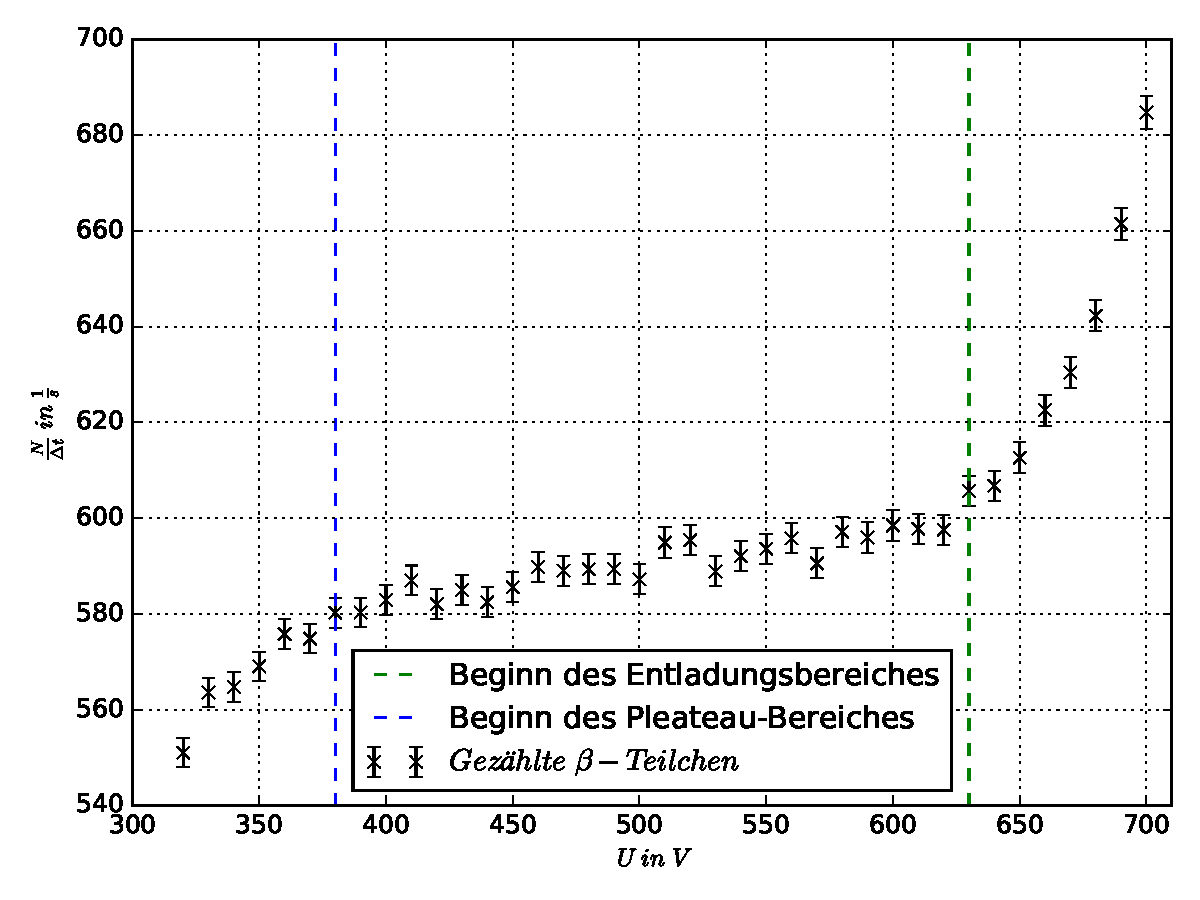
\includegraphics[width=\textwidth]{Charakteristik.pdf}
  \caption{Charakteristik des verwendeten Geiger-Müller-Zählrohres, $\Delta t = \SI{60}{\second}$}
  \label{fig:Charakteristik}
\end{figure}

Die in \ref{fig:Charakteristik} dargestellte Charakteristik zeigt die verwendete
Apparatur bei einer Betriebsspannung zwischen $\num{320}$ bis $\SI{700}{\volt}$.

Die Plateau-Ebene ist deutlich zu erkennen, da in diesem Bereich das Verhältnis zwischen
registrierter Teilchenanzahl pro Minute und der Spannung nahezu konstant ist.
Die Plateau-Ebene beginnt bei ca. $\SI{380}{\volt}$ und endet bei ca.
$\SI{630}{\volt}$.

\begin{figure}
  \centering
  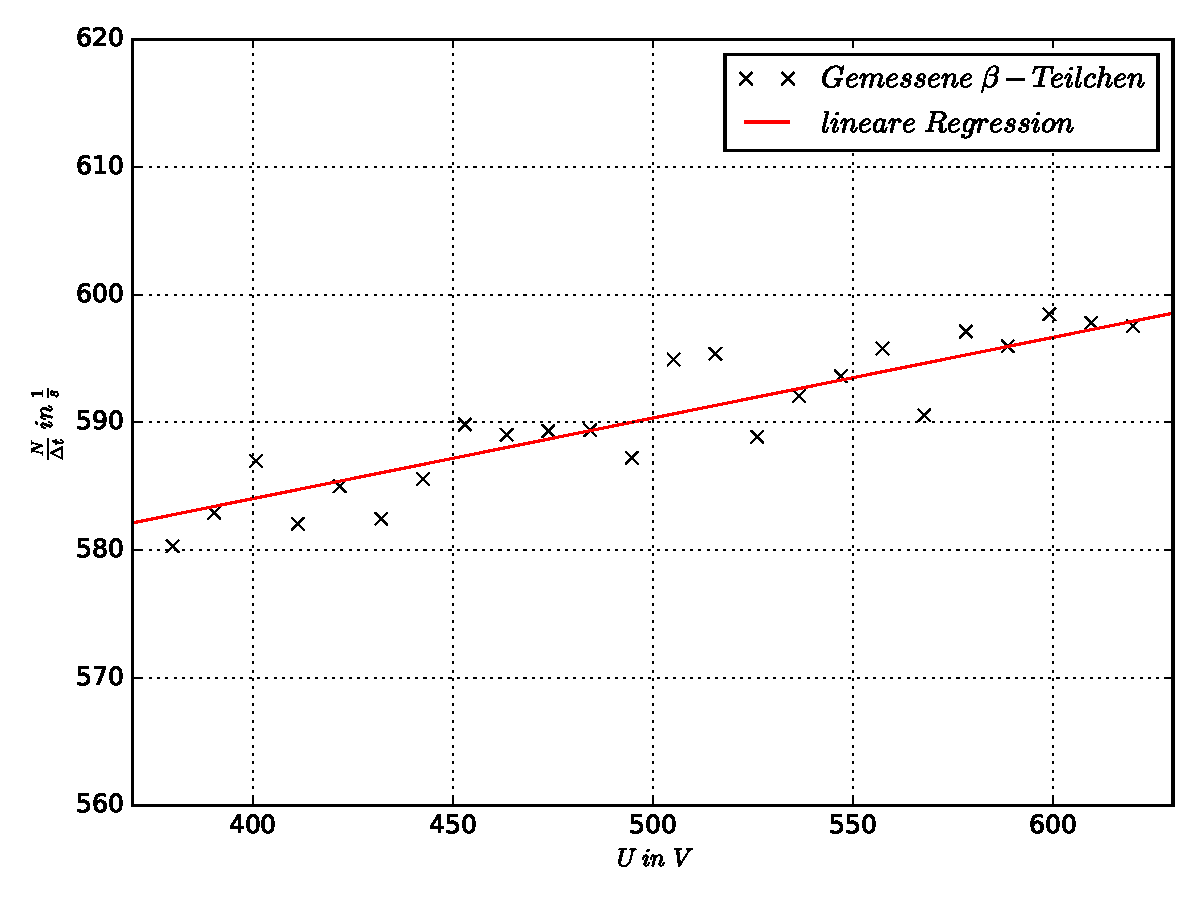
\includegraphics[width=\textwidth]{plateau.pdf}
  \caption{Plateau-Ebene des Messgerätes mit linearer Regression}
  \label{fig:Plateau}
\end{figure}

Die Regressionsgeraden an den Plateau-Bereich hat ungefähr die folgenden Daten.

\begin{equation}
  \label{eqn:function}
  \frac{N}{\Delta t}(U) = \SI{6315e-5}{\per\volt\per\second} \cdot U + \SI{5587e-1}{\per\second}
\end{equation}


Vor der Plateau-Ebene ist der Proportionalitätsbereich von $\SI{320}{\volt}$ bis $\SI{380}{\volt}$ vermessen worden.

An den Plateau-Bereich schließt sich der Entladungsbereich an, der
bis $\SI{700}{\volt}$ gemessen wurde. In diesem Bereich nimmt die
Steigung der registrierten Teilchenanzahl pro Minute im Bezug auf
die angelegte Spannung exponentiell zu.


\subsection{Qualitative Bestimmung der Totzeit}

Die Nachentladungen konnten bei dem Messvorgang der Totzeit $\Tau$, über das
Oszilloskop deutlich beobachtet werden.
Es wurden insgesamt fünf Messungen bei unterschiedlicher Anodenspannung
genommen.


\floatplacement{table}{htbp}
\begin{table}
 \centering
 \caption{Qualitativ bestimmte Totzeit}
 \sisetup{table-format=3.0}
 \begin{tabular}[width=\textwidth]{S S}
     \toprule
   {Spannung in  $\si{\volt}$} & {Totzeit in $\si{\mu\second}$}\\
     \midrule
     400 & 180 \\
     450 & 190 \\
     500 & 200 \\
     550 & 210 \\
     600 & 215 \\
    \bottomrule
\end{tabular}
  \label{tab:Totzeit_1}
\end{table}

Aus den Daten der Tabelle \ref{tab:Totzeit_1} wurde der Mittelwert mit
zugehöriger Standardabweichung bestimmt.
Es ergibt sich der Wert $\Tau = \SI{2.39 (8)}{\mu\second}$.

Gleichzeitig wurde auch die Erholungszeit qualitativ bestimmt.
Die Messergebnisse sind in Tabelle \ref{tab:Erholungszeit} angegeben.

\floatplacement{table}{htbp}
\begin{table}
 \centering
 \caption{Qualitativ bestimmte Totzeit}
 \sisetup{table-format=3.0}
 \begin{tabular}[width=\textwidth]{S S}
     \toprule
   {Spannung in  $\si{\volt}$} & {Erholungszeit in $\si{\milli\second}$}\\
     \midrule
     400 & 2,3 \\
     450 & 2,3 \\
     500 & 2,4 \\
     550 & 2,45 \\
     600 & 2,5 \\
    \bottomrule
\end{tabular}
  \label{tab:Erholungszeit}
\end{table}

Für die Erholungszeit ergibt sich der Wert $t_{\symup{Erholung}} = \SI{2,39(8)}{\milli\second}$.

\subsection{Bestimmung der Totzeit mithilfe der Zwei-Quellen-Methode}

Die wahre Impulsrate $N_{\symup{w}}$ unterscheidet sich aufgrund der Totzeit $\Tau$ von der
gemessenen Impulsrate $N_{\symup{r}}$ um den Faktor $\frac{1}{1-\Tau N_{\symup{r}}}$.

Aus diesem Grund wird die Zwei-Quellen-Methode verwendet, bei der
zuerst die Impulsrate einer einzelnen Quelle gemessen wird.
Daraufhin wird eine weitere Quelle hinzugefügt, die eine unterschiedliche
Strahlungsrate besitzt. Im letzten Schritt wird die erste Quelle aus der
Apparatur entnommen.

Aufgrund der genommenen Messwerte kann die Totzeit für $\Tau^2N_{\symup{i}}^2 << 1$
($i = 1, 2, 1+2$) durch die Formel \eqref{eqn:Totzeit} approximiert werden.

\begin{equation}
  \label{eqn:Totzeit}
  \Tau \approx \frac{N_1 + N_2 - N_{1+2}}{2N_1N_2}
\end{equation}

Die Messung ergaben die folgenden Werte.

\begin{description}
  \item[$N_1:$] 25692
  \item[$N_2:$] 1109
  \item[$N_{1+2}:$] 26775
\end{description}

Dabei sind die $N_i$ ($i = 1, 2, 1+2$) in registrierten Teilchen pro Minute bestimmt.

Aus den Messwerten ergibt sich mit der Formel \eqref{eqn:Totzeit}
$\Tau$ zu \SI{3(24)e-5}{\second}.

\subsection{Messung der pro Teilchen vom Zählrohr freigesetzten Ladungsmenge}

In dem Versuch wurde der vom Zählrohr freigesetzte Strom
in Abhängigkeit von der angelegten Spannung gemessen.
Die Messung wurde in $\SI{10}{\volt}$ Schritten von
$\SI{320}{\volt}$ bis $\SI{700}{\volt}$ durchgeführt.
Die Messdaten sind in Tabelle \ref{tab:Charakteristik} dargestellt.
Zwischen der Zählrate und der gemessenen Stromstärke besteht ein
linearer Zusammenhang der wie folgt dazustellen ist.

\begin{equation*}
  I = \Delta Q \cdot N
\end{equation*}

Deshalb lässt sich die freigesetzte Ladung por Teilchen im Zählrohr über eine
lineare Regression aus den Daten der Tabelle \ref{tab:Charakteristik} ermitteln.
Dafür wurde die gemessene Stromstärke der registrierte Teilchenanzahl pro Minute
gegenübergestellt.

\begin{figure}
  \centering
  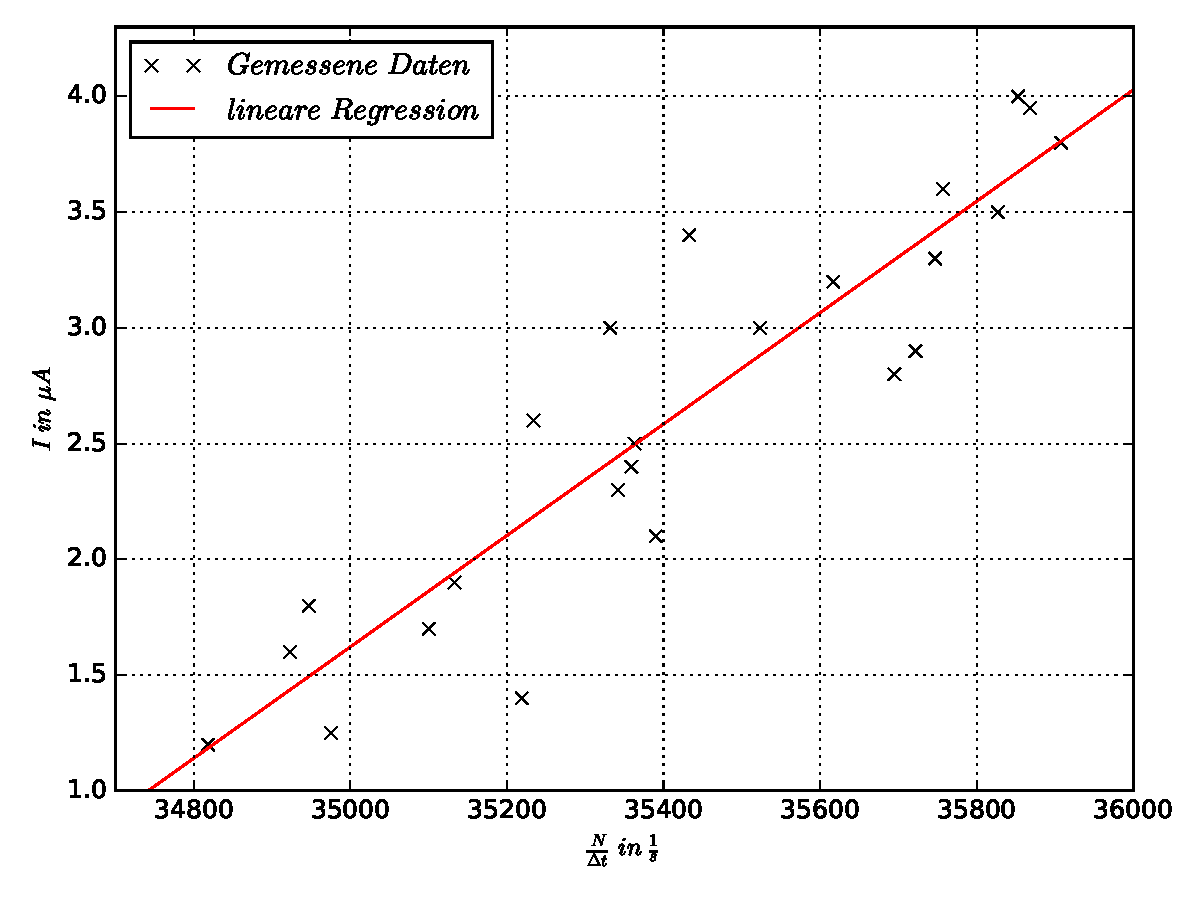
\includegraphics[width=\textwidth]{Stromstärke_gegen_Anzahl.pdf}
  \caption{Gemessenen Stromstärke gegenüber der Teilchenanzahl pro Minute mit linearer Regression}
  \label{fig:Stromstärke_gegen_Anzahl}
\end{figure}

Die Ausgleichsgerade hat ungefähr die folgenden Daten.

\begin{equation}
  \label{eqn:Augleichsgerade_Ladung}
  I(N) = \SI{2406(223)e-3}{\mu\ampere\second}\cdot N - \SI{82,577(8)}{\coulomb}
\end{equation}

Die Ladung pro Teilchen ist ungefähr gleich der Steigung der Ausgleichsgeraden.
Damit wird jedem Teilchen eine freigesetzte Ladungsmende von $\approx \SI{2,406e-3}{\coulomb}$
zugeordnet. Dies entspricht ca. $\num{1,502e16}$ Elementarladungen.

Zudem wurde die Stromstärke bei steigender SPannung gemessen. Das Messintervall
erstreckt sich über den selben Spannungsbereich wie bei Bestimmung der Charakteristik.

Eine Grafik dieses Diagrammes ist in Abb. \ref{fig:Spannung gegen Strom}
dargestellt.

\begin{figure}
  \centering
  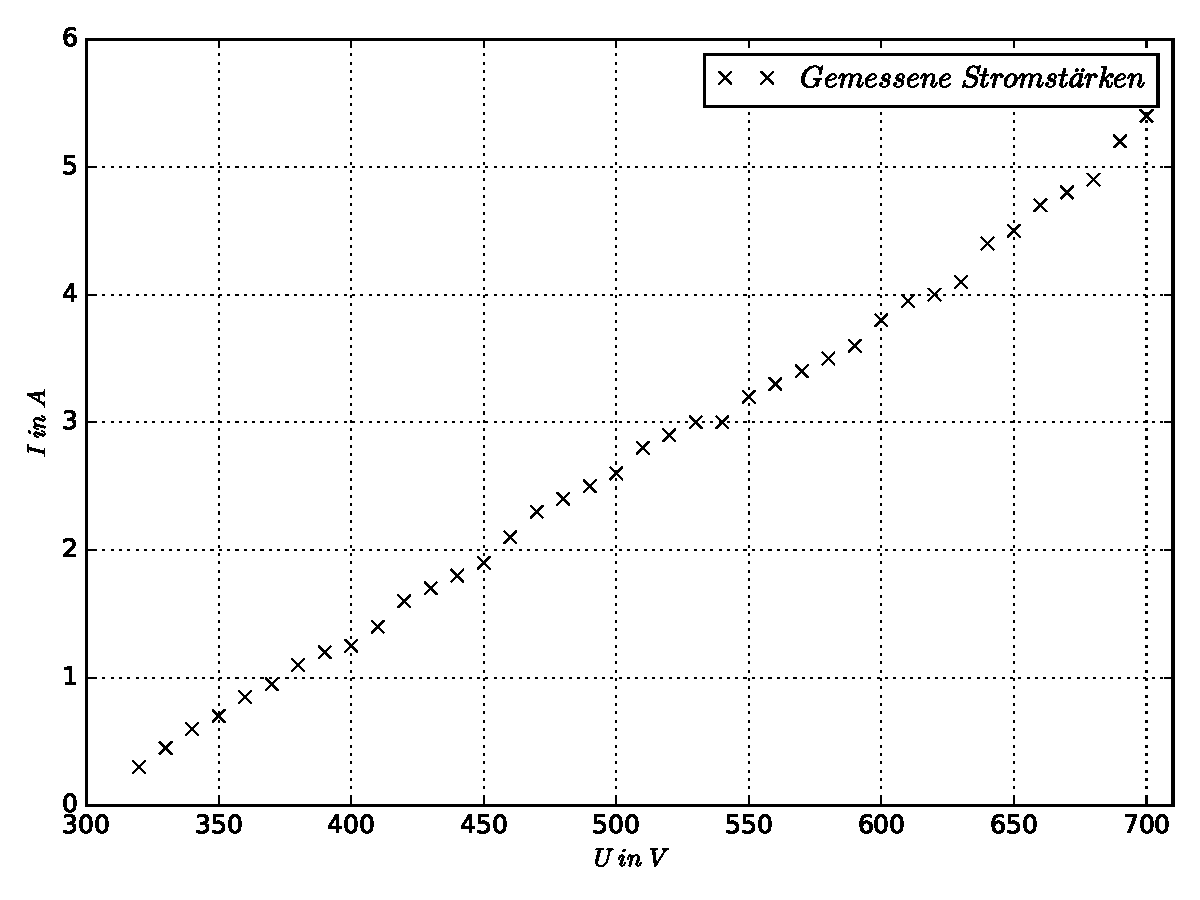
\includegraphics[width=\textwidth]{Spannung_gege_Strom.pdf}
  \caption{Gemessenen Stromstärke gegenüber der Spannung}
  \label{fig:Spannung gegen Strom}
\end{figure}

Anhand der Abb. \ref{fig:Spannung gegen Strom} wird ersichtlich, dass die Stromstärke
mit zunehmender Spannung ebenfalls zunimmt. Der Zusammenhang scheint linear.

\section{Diskussion}

Die Steigung der Regressiongeraden, die an die Plateau-Ebene angelegt wurde
besitzt eine sehr geringe Steigung (vgl. \ref{eqn:function}).
Damit ist das Verhältnis zwischen registriertet Teilchenanzahl und Spannung
im Rahmen der Messgenauigkeit als konstant anzusehen. Insgesamt werden
an der aufgenommenen Charakteristik die grundsätzlichen Merkmale eines
Geiger-Müller-Zählrohres deutlich ersichtlich.

Die Totzeit konnte an der verwendeten Apparatur nicht über die Zwei-Quellen-Methode
bestimmt werden, da die Probenhalterung beim einlegen der zweiten Quelle
verwackelt ist, sodass keine zuverlässigen Messwerte erhoben werden konnten.
Die verwendeten Messdaten entstammen den Messungen der parallel arbeitenden
Gruppe Steven D. Becker und Stefan G. Grisard.
Deshalb ist der Vergleich zwischen den Methoden zur Bestimmung der Totzeit
nicht sinnvoll. Es wird angenommen, dass die qualitativ bestimmte
Totzeit tatsächlich die Totzeit der Apparatur genügend gut beschreibt.

Die Messung der pro Teilchen vom Zählrohr freigesetzten Ladungsmenge wurde mithilfe
einer linearen Regression bewerkstelligt. Dies ist sinnvoll, da ein linearer
Zusammenhang zwischen der registrierten Teilchenanzahl pro Minute und der
währenddessen gemessenen Stromstärke bestehnt.
Der Porportionalitätsfaktor zwischen den beiden Größen ist die freigesetzte
Ladung. Es wurde ledignlich der Plateau-Bereich betrachtet, da davon auszugehen
ist, dass dort die Nachentladungen vernachlässigbar gering sind und die
freigesetzte Ladungsmenge lediglich von der Anfangsenergie des eingehenden
Teilchen stammt. Damit lässt sich dann die freigesetzte Ladungsmenge pro Teilchen
möglichst präzise bestimmen.


\section{Messdaten}

In diesem Kapitel sind die Messdaten der Messung der Charakteristik dargestellt.





%\floatplacement{table}{htbp}
%\begin{table}
% \centering
% \caption{Messdaten zur Charakteristik}
% \begin{tabular}[width=\textwidth]{S S S}
%     \toprule
%   {Spannung in  $\si{volt}$} & {Zählrate in $\frac{1}{\si{\minute}}$} & %{Stromstärke in $\si{\milli\ampere}$}\\
%     \midrule
%     320 & 33062 & 0,3 \\
%     330 & 33816 & 0,45 \\
%     340 & 33883 & 0,6 \\
%     350 & 34142 & 0,7 \\
%     360 & 34549 & 0,85 \\
%     370 & 34491 & 0,95 \\
%     380 & 34815 & 1,1 \\
%     390 & 34818 & 1,2 \\
%     400 & 34975 & 1,25 \\
%     410 & 35219 & 1,4 \\
%     420 & 34923 & 1,6 \\
%     430 & 35100 & 1,7 \\
%     440 & 34947 & 1,8 \\
%     450 & 35133 & 1,9 \\
%     460 & 35390 & 2,1 \\
%     470 & 35342 & 2,3 \\
%     480 & 35359 & 2,4 \\
%     490 & 35363 & 2,5 \\
%     500 & 35234 & 2,6 \\
%     510 & 35695 & 2,8 \\
%     520 & 35722 & 2,9 \\
%     530 & 35332 & 3,0 \\
%     540 & 35523 & 3,0 \\
%     550 & 35617 & 3,2 \\
%     560 & 35747 & 3,3 \\
%     570 & 35433 & 3,4 \\
%     580 & 35827 & 3,5 \\
%     590 & 35757 & 3,6 \\
%     600 & 35908 & 3,8 \\
%     610 & 35868 & 3,95 \\
%     620 & 35853 & 4,0 \\
%     630 & 36340 & 4,1 \\
%     640 & 36405 & 4,4 \\
%     650 & 36758 & 4,5 \\
%     660 & 37352 & 4,7 \\
%     670 & 37824 & 4,8 \\
%     680 & 38535 & 4,9 \\
%     690 & 39689 & 5,2 \\
%     700 & 41082 & 5,4 \\
%    \bottomrule
%\end{tabular}
%  \label{tab:Charakteristik}
%\end{table}

\input{"Tabelle_Charakteristik.tex"}

\end{document}
